\documentclass[english,floatsintext,man]{apa6}

\usepackage{amssymb,amsmath}
\usepackage{ifxetex,ifluatex}
\usepackage{fixltx2e} % provides \textsubscript
\ifnum 0\ifxetex 1\fi\ifluatex 1\fi=0 % if pdftex
  \usepackage[T1]{fontenc}
  \usepackage[utf8]{inputenc}
\else % if luatex or xelatex
  \ifxetex
    \usepackage{mathspec}
    \usepackage{xltxtra,xunicode}
  \else
    \usepackage{fontspec}
  \fi
  \defaultfontfeatures{Mapping=tex-text,Scale=MatchLowercase}
  \newcommand{\euro}{€}
\fi
% use upquote if available, for straight quotes in verbatim environments
\IfFileExists{upquote.sty}{\usepackage{upquote}}{}
% use microtype if available
\IfFileExists{microtype.sty}{\usepackage{microtype}}{}

% Table formatting
\usepackage{longtable, booktabs}
\usepackage{lscape}
% \usepackage[counterclockwise]{rotating}   % Landscape page setup for large tables
\usepackage{multirow}		% Table styling
\usepackage{tabularx}		% Control Column width
\usepackage[flushleft]{threeparttable}	% Allows for three part tables with a specified notes section
\usepackage{threeparttablex}            % Lets threeparttable work with longtable

% Create new environments so endfloat can handle them
% \newenvironment{ltable}
%   {\begin{landscape}\begin{center}\begin{threeparttable}}
%   {\end{threeparttable}\end{center}\end{landscape}}

\newenvironment{lltable}
  {\begin{landscape}\begin{center}\begin{ThreePartTable}}
  {\end{ThreePartTable}\end{center}\end{landscape}}




% The following enables adjusting longtable caption width to table width
% Solution found at http://golatex.de/longtable-mit-caption-so-breit-wie-die-tabelle-t15767.html
\makeatletter
\newcommand\LastLTentrywidth{1em}
\newlength\longtablewidth
\setlength{\longtablewidth}{1in}
\newcommand\getlongtablewidth{%
 \begingroup
  \ifcsname LT@\roman{LT@tables}\endcsname
  \global\longtablewidth=0pt
  \renewcommand\LT@entry[2]{\global\advance\longtablewidth by ##2\relax\gdef\LastLTentrywidth{##2}}%
  \@nameuse{LT@\roman{LT@tables}}%
  \fi
\endgroup}


  \usepackage{graphicx}
  \makeatletter
  \def\maxwidth{\ifdim\Gin@nat@width>\linewidth\linewidth\else\Gin@nat@width\fi}
  \def\maxheight{\ifdim\Gin@nat@height>\textheight\textheight\else\Gin@nat@height\fi}
  \makeatother
  % Scale images if necessary, so that they will not overflow the page
  % margins by default, and it is still possible to overwrite the defaults
  % using explicit options in \includegraphics[width, height, ...]{}
  \setkeys{Gin}{width=\maxwidth,height=\maxheight,keepaspectratio}
\ifxetex
  \usepackage[setpagesize=false, % page size defined by xetex
              unicode=false, % unicode breaks when used with xetex
              xetex]{hyperref}
\else
  \usepackage[unicode=true]{hyperref}
\fi
\hypersetup{breaklinks=true,
            pdfauthor={},
            pdftitle={On the Origin of the Matthew Effect: Insights from a Quantitative Theoretical Model},
            colorlinks=true,
            citecolor=blue,
            urlcolor=blue,
            linkcolor=black,
            pdfborder={0 0 0}}
\urlstyle{same}  % don't use monospace font for urls

\setlength{\parindent}{0pt}
%\setlength{\parskip}{0pt plus 0pt minus 0pt}

\setlength{\emergencystretch}{3em}  % prevent overfull lines

\ifxetex
  \usepackage{polyglossia}
  \setmainlanguage{}
\else
  \usepackage[english]{babel}
\fi

% Manuscript styling
\captionsetup{font=singlespacing,justification=justified}
\usepackage{csquotes}
\usepackage{upgreek}



\usepackage{tikz} % Variable definition to generate author note

% fix for \tightlist problem in pandoc 1.14
\providecommand{\tightlist}{%
  \setlength{\itemsep}{0pt}\setlength{\parskip}{0pt}}

% Essential manuscript parts
  \title{On the Origin of the Matthew Effect: Insights from a Quantitative
Theoretical Model}

  \shorttitle{Origin}


  \author{Matthew T. McBee\textsuperscript{1}, Matthew C. Makel\textsuperscript{2}, \& Natasha L. Godkin\textsuperscript{1}}

  \def\affdep{{"", "", ""}}%
  \def\affcity{{"", "", ""}}%

  \affiliation{
    \vspace{0.5cm}
          \textsuperscript{1} East Tennessee State University\\
          \textsuperscript{2} Duke University Talent Identification Program  }

 % If no author_note is defined give only author information if available
      \newcounter{author}
                              \authornote{
            Correspondence concerning this article should be addressed to Matthew T. McBee. E-mail: \href{mailto:mcbeem@etsu.edu}{\nolinkurl{mcbeem@etsu.edu}}
          }
                                                

  \abstract{A quantitative theoretical model of academic achievement, based on the
concept of the Zone of Proximal Development (ZPD), has proven capable of
reproducing the results of several empirical, longitudinal studies of
achievement. This paper applies the model to understanding the origins
of variance in achievement (at the individual and subgroup mean level of
analysis), and the effect of gifted education initiatives on that
variability.}
  \keywords{gifted, excellence gap, zone of proximal development, theoretical
calculation \\

    \indent Word count: X
  }





\usepackage{amsthm}
\newtheorem{theorem}{Theorem}
\newtheorem{lemma}{Lemma}
\theoremstyle{definition}
\newtheorem{definition}{Definition}
\newtheorem{corollary}{Corollary}
\newtheorem{proposition}{Proposition}
\theoremstyle{definition}
\newtheorem{example}{Example}
\theoremstyle{definition}
\newtheorem{exercise}{Exercise}
\theoremstyle{remark}
\newtheorem*{remark}{Remark}
\newtheorem*{solution}{Solution}
\begin{document}

\maketitle

\setcounter{secnumdepth}{0}



\section{Theoretical Framework}\label{theoretical-framework}

Current educational and psychological theories, being qualitative, are
incapable of generating precise quantitative predictions --
\enquote{point predictions} -- that are the hallmark of the physical
sciences (c.f. Cohen, 1994; Maxwell \& Howard, 2009; Meehl, 1967). For
theories to be falsifiable, they must make specific predictions. Only
then can empirical research provide the type of severe tests (Mayo,
1996) that lead to meaningful scientific progress. We propose such a
theory in this paper. Our theory of academic achievement growth can
describe and predict the achievement trajectories of individual
students, accounting for both individual and environmental factors.

\section{Methods1}\label{methods1}

The Zone of Proximal Development (ZPD) is the basic psychological
principle at the heart of this theoretical model. Although the ZPD
concept is typically attributed to Lev Vygotsky, the phenomenon was
actually first revealed by Dorthea McCarthy (1930). The ZPD describes
how learning emerges from the interaction between a student's base of
currently mastered skills and knowledge with a particular set of
learning experiences, and refers specifically to the set of skills that
a student cannot perform autonomously but can do with scaffolding from a
teacher or more competent peer. In our theory, instruction that occurs
within the ZPD leads to the most rapid, efficient learning.

\subsection{Academic achievement}\label{academic-achievement}

We define the term academic achievement to mean a student's location
along a sequenced, developmental curriculum within a specific domain.
Academic achievement therefore refers to the body of knowledge,
understanding, and skills that a student has mastered at a particular
moment in time. Academic growth or achievement growth is change
(typically positive) in achievement over time. Our numeric scale for
measuring achievement ranges from zero to positive infinity, where zero
is a meaningful quantity representing no knowledge or skills in the
domain. Specific values of achievement could refer to the location of
specific skill milestones or content mastery. For example, one could
(arbitrarily) set the mastery of mathematical operations expected of a
typical third grader to a value of 0.40 on the achievement metric. ZPD.
The ZPD is represented by a normal curve, normalized to a maximum value
of one, whose peak is slightly ahead of the student's current
achievement (Figure 1). In the figure, a vertical line at 0.25 depicts
the student's current achievement; her ZPD is the shaded curve peaking
at 0.30. The ZPD is not a single point but rather a \enquote{spread} of
values varying in intensity; its peak describes the most efficacious
level of instruction for stimulating academic growth.

Insert Figure 1 here

\subsection{School curriculum.}\label{school-curriculum.}

School curriculum is co-located on the same scale with academic
achievement in much the same way that IRT models place test scores and
item difficulties on a common scale. For example, one could imagine that
a typical Kindergarten reading curriculum ranges from 0.05 to 0.15,
where 0.05 might include basic letter and phoneme awareness and 0.15 a
limited ability to \enquote{sound out} simple words and knowledge of
roughly 200 sight words. Within this academic year, the curriculum
presented on a specific day would consist of a narrow slice or segment
of this interval, and as the year progresses, the presented curriculum
would steadily advance. Our model uses a normalized trapezoidal
distribution to represent the school curriculum due to the many shapes
it can assume with different choices of values for its parameters.
Figure 2 illustrates how three students, with varying initial
achievement, can experience the same school curriculum. Only the student
in the center panel would derive strong benefit from exposure to this
curriculum as it falls within his ZPD. The curriculum is too difficult
for the first student and too easy for the third; neither of these
students would experience much benefit. Our implementation of the model
in our R package does allow for students to experience different
curricula (e.g., remedial, typical, or advanced) on an individual basis.

Insert Figure 2 here

\subsection{Home curriculum}\label{home-curriculum}

Children learn a great deal at home, particularly in early childhood and
in certain subjects such as reading. The rate of academic growth caused
by learning experiences at home is a function of the overlap between the
child's ZPD and what we call the \enquote{home curriculum}, which we
conceptualize as a downward-sloping function. Our R package implantation
represents the home curriculum as a normalized beta distribution with
the \(\alpha\) parameter fixed to 1. Figure 3 displays the home
curriculum function (with parameter \(\beta\) set to 5) with a
superimposed ZPD for a child with achievement = 0.20. The implication of
this downward slope is that academic growth due to home instruction is
most rapid in early childhood and becomes increasingly reliant on school
instruction in later grades.

Insert Figure 3 here

\subsection{Individual difference
parameters}\label{individual-difference-parameters}

Our model incorporates four child-level parameters: current achievement,
learning rate, decay rate, and home environment; these create
variability in growth trajectories. The learning rate represents
individual differences in the pace of academic growth for students with
identical levels of ZPD engagement, and can be considered to be a
combination of general intelligence and motivation. The decay rate is
the rate at which achievement will decay (due to forgetting) in the
absence of instruction. The home environment parameter describes how
effectively the home environment is at facilitating academic growth.

\subsection{Model dynamics}\label{model-dynamics}

The amount of learning during discrete time interval \(t\) for
individual \(i\) is given by

\begin{equation}
\begin{split}
\textit{Learning}_{ti} = \textit{LearnRate}_i \, &* \\
  & \big[ \big( \textit{dosage}_{ti} * \int_{0}^{\infty} \textit{ZPD}_{ti}(x) * S_t(x) \, dx \big) + \\ 
  & (1-\textit{dosage}_{ti}) * \textit{HomeEnv}_i * \int_{0}^{\infty} \textit{ZPD}_{ti}(x) * H_t(x) \, dx \big) \big]
\end{split}
\end{equation}

\begin{figure}[htbp]
\centering
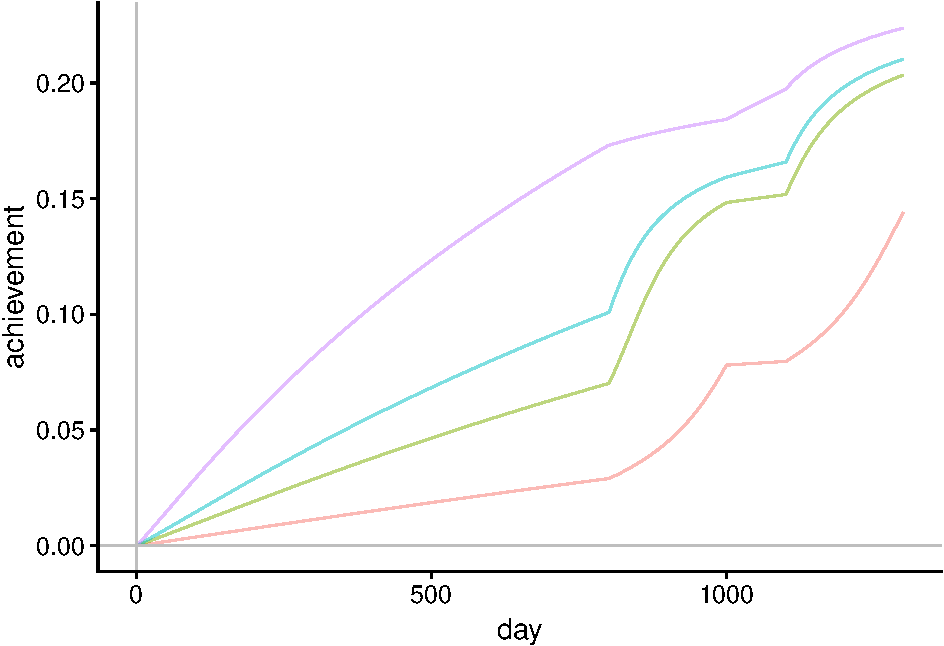
\includegraphics{Matthew_effect_origin_AERA2018_files/figure-latex/unnamed-chunk-3-1.pdf}
\caption{}
\end{figure}

\begin{figure}[htbp]
\centering
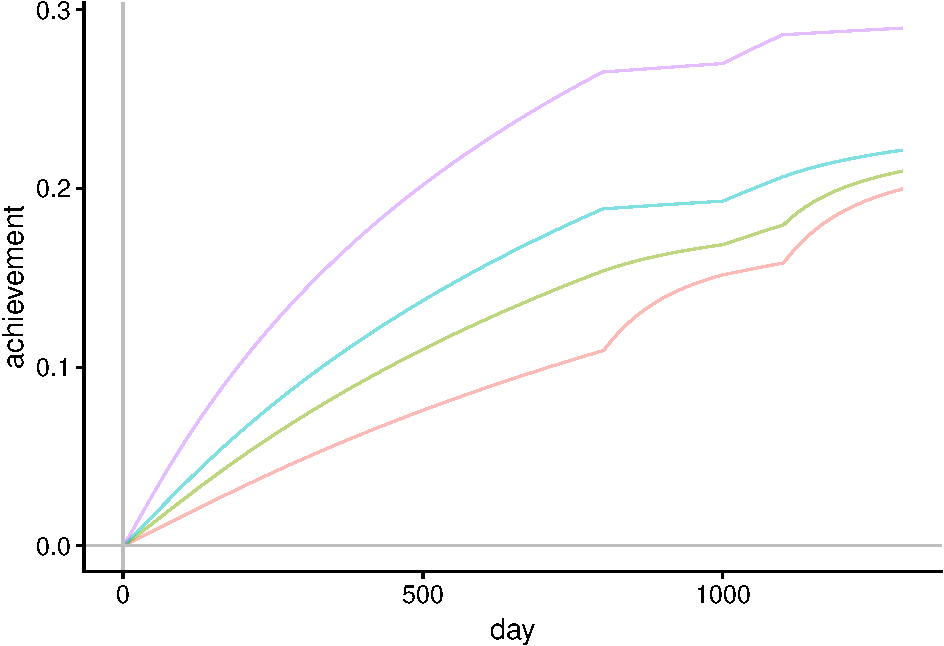
\includegraphics{Matthew_effect_origin_AERA2018_files/figure-latex/unnamed-chunk-4-1.pdf}
\caption{}
\end{figure}

\begin{figure}[htbp]
\centering
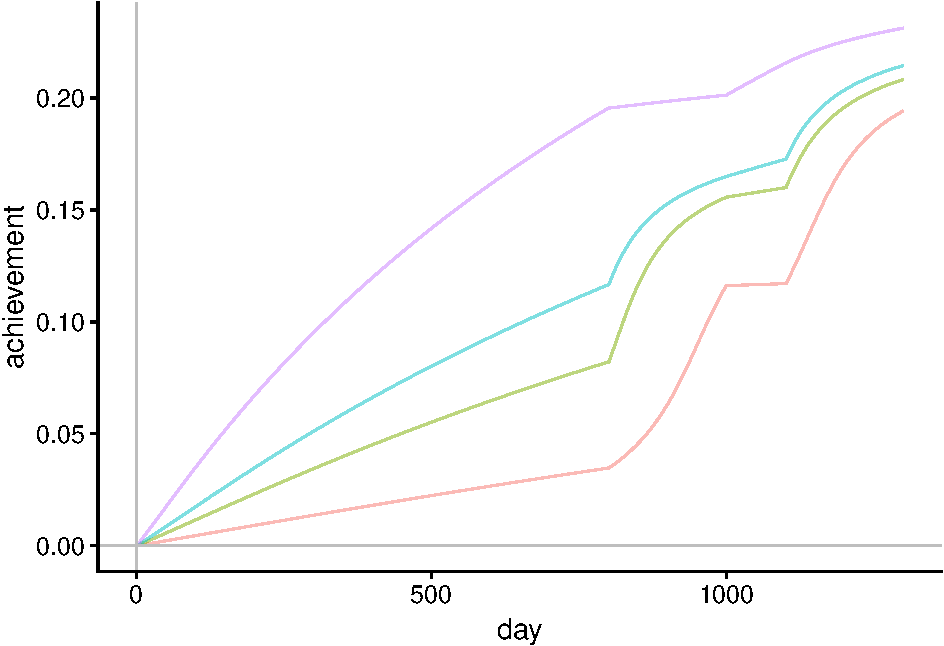
\includegraphics{Matthew_effect_origin_AERA2018_files/figure-latex/unnamed-chunk-5-1.pdf}
\caption{}
\end{figure}

\begin{figure}[htbp]
\centering
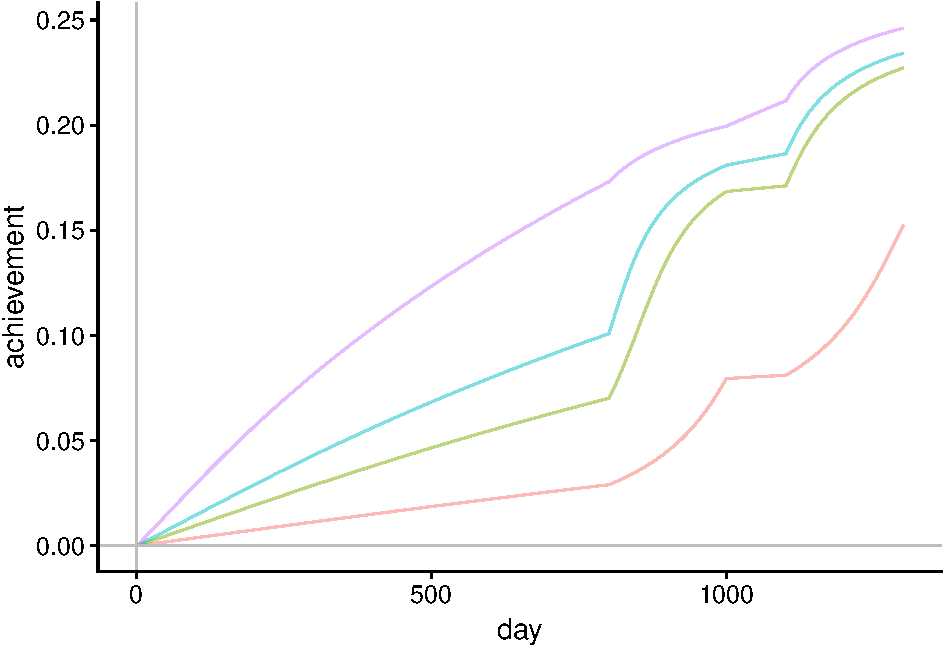
\includegraphics{Matthew_effect_origin_AERA2018_files/figure-latex/unnamed-chunk-6-1.pdf}
\caption{}
\end{figure}

\begin{figure}[htbp]
\centering
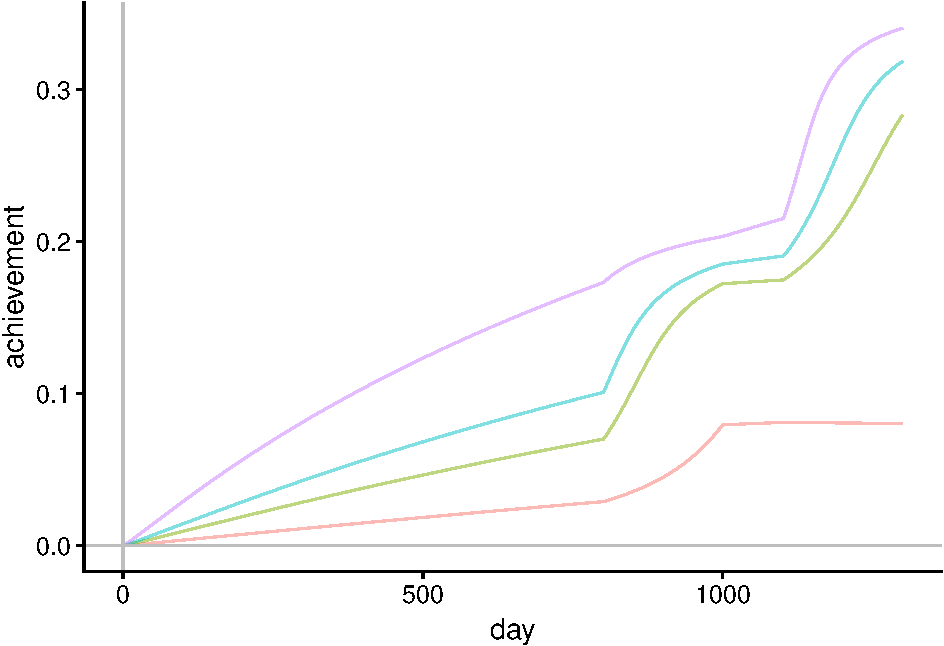
\includegraphics{Matthew_effect_origin_AERA2018_files/figure-latex/unnamed-chunk-7-1.pdf}
\caption{}
\end{figure}

\section{Methods}\label{methods}

We report how we determined our sample size, all data exclusions (if
any), all manipulations, and all measures in the study.

\subsection{Participants}\label{participants}

\subsection{Material}\label{material}

\subsection{Procedure}\label{procedure}

\subsection{Data analysis}\label{data-analysis}

We used R (3.4.0, R Core Team, 2017) and the R-packages \emph{cowplot}
(0.9.2, Wilke, 2017), \emph{dplyr} (0.7.4, Wickham, Francois, Henry, \&
Müller, 2017), \emph{ggplot2} (2.2.1, Wickham, 2009), \emph{papaja}
(0.1.0.9492, Aust \& Barth, 2017), and \emph{ZPDGrowthTrajectories}
(0.0.5, McBee, 2017) for all our analyses.

\section{Results}\label{results}

\section{Discussion}\label{discussion}

\newpage

\section{References}\label{references}

\setlength{\parindent}{-0.5in} \setlength{\leftskip}{0.5in}

\hypertarget{refs}{}
\hypertarget{ref-R-papaja}{}
Aust, F., \& Barth, M. (2017). \emph{papaja: Create APA manuscripts with
R Markdown}. Retrieved from \url{https://github.com/crsh/papaja}

\hypertarget{ref-R-ZPDGrowthTrajectories}{}
McBee, M. (2017). \emph{ZPDGrowthTrajectories: Simulates achievement
growth trajectories using a theoretical model of academic achievement}.

\hypertarget{ref-R-base}{}
R Core Team. (2017). \emph{R: A language and environment for statistical
computing}. Vienna, Austria: R Foundation for Statistical Computing.
Retrieved from \url{https://www.R-project.org/}

\hypertarget{ref-R-ggplot2}{}
Wickham, H. (2009). \emph{Ggplot2: Elegant graphics for data analysis}.
Springer-Verlag New York. Retrieved from \url{http://ggplot2.org}

\hypertarget{ref-R-dplyr}{}
Wickham, H., Francois, R., Henry, L., \& Müller, K. (2017). \emph{Dplyr:
A grammar of data manipulation}. Retrieved from
\url{https://CRAN.R-project.org/package=dplyr}

\hypertarget{ref-R-cowplot}{}
Wilke, C. O. (2017). \emph{Cowplot: Streamlined plot theme and plot
annotations for 'ggplot2'}. Retrieved from
\url{https://CRAN.R-project.org/package=cowplot}






\end{document}
